%\documentclass[11pt]{beamer}
\documentclass{beamer}
%\newcommand\Fontvi{\fontsize{6}{7.2}\selectfont}
\usepackage{caption}
%\captionsetup{font+=scriptsize}
\usepackage{pgffor}
\usepackage{verbatim}
\usepackage[T1]{fontenc}
\catcode`\_=12

\newcommand\Fontvi{\fontsize{6}{7.2}\selectfont}
\newcommand\vtiny{\fontsize{2}{3}\selectfont}
\newcommand{\inputpath}[1]{}
\newcommand{\feat}{dummy}
\newcommand{\plategroup}{dummy}
\newcommand{\reptype}{dummy}
\newcommand{\sha}{dummy}
 \usepackage{multimedia}
 \usepackage{xmpmulti}
 %\usepackage{pgf,pgfarrows,pgfnodes,pgfautomata,pgfheaps,pgfshade}
 \usepackage{amsmath,amssymb}
 \usepackage[latin1]{inputenc}
 \usepackage{colortbl}
 %\usepackage{babel}
 \usepackage{multimedia}
 \usepackage{times}
 \usepackage{hyperref}
 \usepackage{dsfont}
 \usepackage{verbatim}
\DeclareGraphicsExtensions{.pdf,.png}


\definecolor{darkgreen}{rgb}{0,0.4,0}
\definecolor{darkblue}{rgb}{0,0,0.4}

 \newcommand{\hatW}{\widehat{\Delta}}
 \newcommand{\hatu}{\widehat{u}}
 \newcommand{\varu}{\widehat{\upsilon}}
 \newcommand{\bu}{\widehat{b}}
 \newcommand{\Wni}{\widehat{n}(\x_i)}
 \newcommand{\Wnj}{\widehat{n}(\x_j)}
 \newcommand{\sigu}{\widehat{\sigma}}
 \newcommand{\Ast}{\star}
 \newcommand{\Wuo}{\Delta^\Ast}
 \newcommand{\hatuo}{u ^\Ast}
 \newcommand{\Wnuoi}{n^\Ast(\x_i)}
 \newcommand{\varuo}{\upsilon^\Ast}
 \newcommand{\stduo}{{\upsilon^2}^\Ast}
 \newcommand{\buo}{b^\Ast}
 \newcommand{\ruo}{r^\Ast}
 \newcommand{\Domain}{G}
 \newcommand{\residual}{r}
 \newcommand{\x}{{\bf x}}
 \newcommand{\setW}{{\cal H}_{\Delta}}
 \newcommand{\Sim}{\sim}
 \newcommand{\E}{{\mathbb E}}
 \newcommand{\R}{{\mathbb R}}
 \newcommand{\Proba}{\mathbb{P}}
 \newcommand{\eps}{\varepsilon}
 \newcommand{\calH}{{\cal H}}
 \newtheorem{proposition}{Proposition}
 \newcommand{\refe}[1]{[{\em #1}]}
 
 \newcommand{\eqn}[1]{eqn.~\ref{#1}}
\newcommand{\Sec}[1]{Section~\ref{#1}}
\newcommand{\Chap}[1]{Chapter~\ref{#1}}
\newcommand{\Fig}[1]{Fig.~\ref{#1}}
\newcommand{\App}[1]{Appendix~\ref{#1}}
\newcommand{\Algo}[1]{Algorithm~\ref{#1}}


\newcommand{\figwidth}{40pt}
\newcommand{\platesize}{60pt}
\newcommand{\cmatsize}{90pt}

\setbeamertemplate{caption}[numbered]
\setbeamerfont{caption}{size=\scriptsize}


\makeatletter
    \newenvironment{withoutheadline}{
        \setbeamertemplate{headline}[default]
        \def\beamer@entrycode{\vspace*{-\headheight}}
    }{}
\makeatother


%
 \title[] % (optional, use only with long paper titles)
 {Subpop Analysis log}
 \author[] % (optional, use only with lots of authors)
 {}
 \institute[] % (optional, but mostly needed)
 {Updated Apr 17, 2014}
 \date[]{} % (optional)

\begin{document}
%-----------------------------
\begin{frame}
  \titlepage
\end{frame}
%-----------------------------

%-----------------------------
\frame{
\frametitle{Apr 17, 2015}
}
%-----------------------------
%-----------------------------
\frame{
\frametitle{Summary}
\begin{itemize}
\item We tested classification accuracy using Naive Bayes with and without 
interphase. 
\item Conclusion: At least with Naive Bayes, it doesn't seem to make much of a 
difference.
\end{itemize}
}
%-----------------------------

%-----------------------------
\renewcommand{\sha}{d2255b5a_with_interphase}
\graphicspath{{../results/master/\sha/}}
%-----------------------------
%-----------------------------
\frame{
\frametitle{Counts}
\begin{figure}
    \centering
	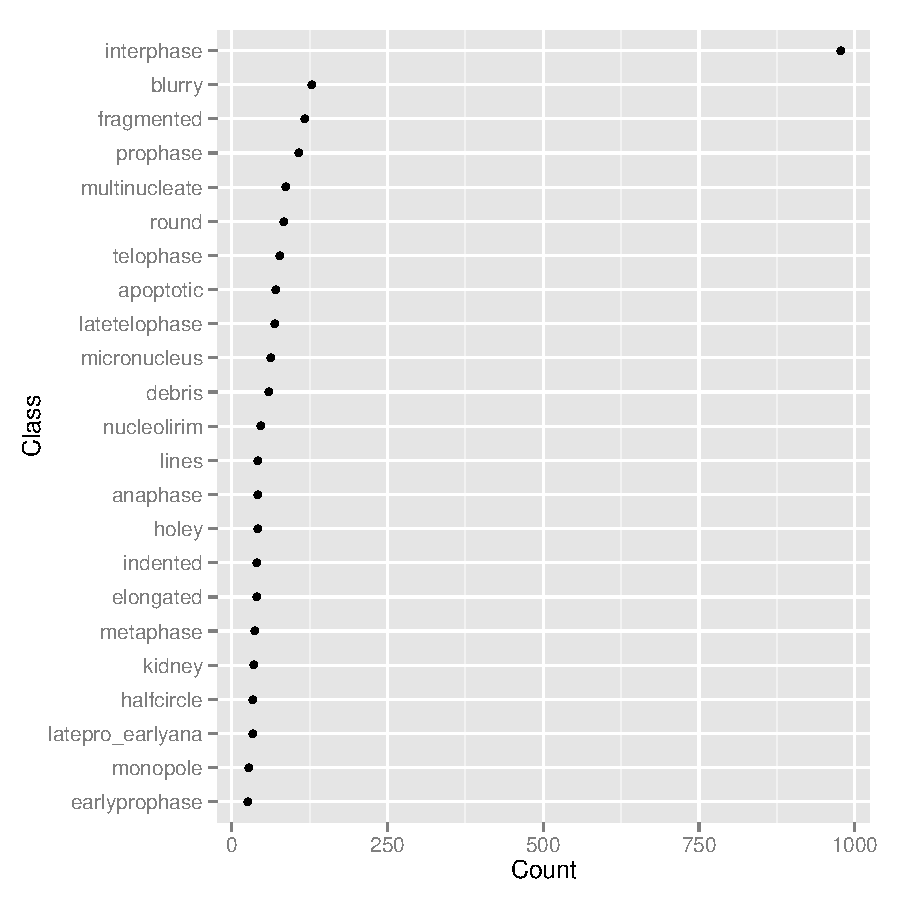
\includegraphics[width=0.8\linewidth]{counts.pdf}
\end{figure}
}
%-----------------------------
%-----------------------------
\frame{
\frametitle{\sha}
\begin{figure}
    \centering
	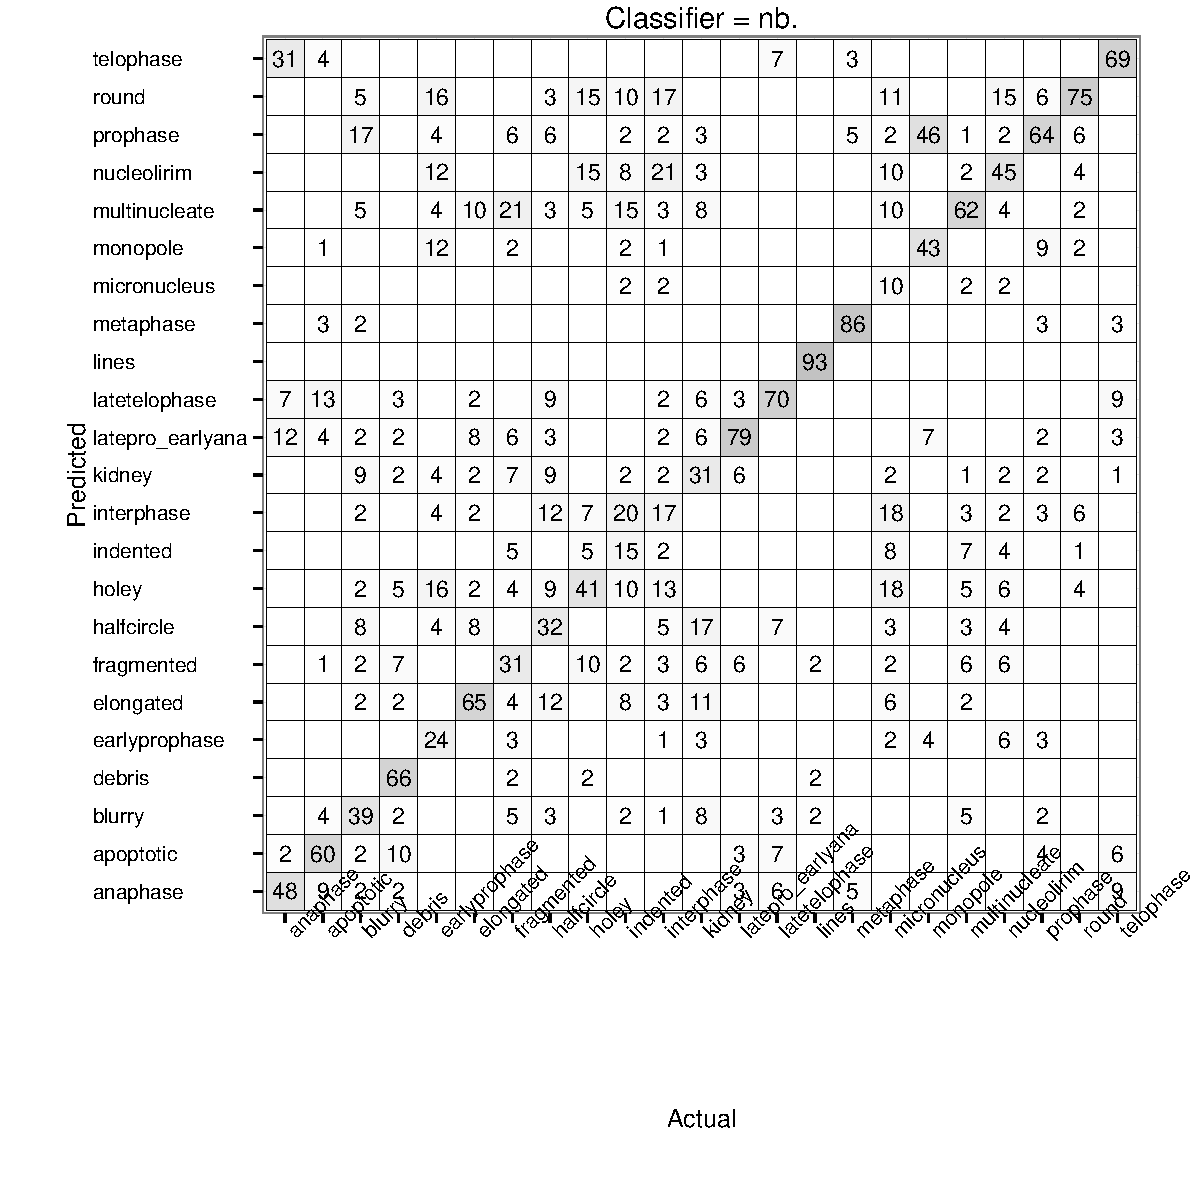
\includegraphics[width=0.8\linewidth]{confmat_loocv_nb.pdf}
\end{figure}
}
%-----------------------------
%-----------------------------
\renewcommand{\sha}{23be6f06_without_interphase}
\graphicspath{{../results/master/\sha/}}
%-----------------------------
%-----------------------------
\frame{
\frametitle{\sha }
\begin{figure}
    \centering
	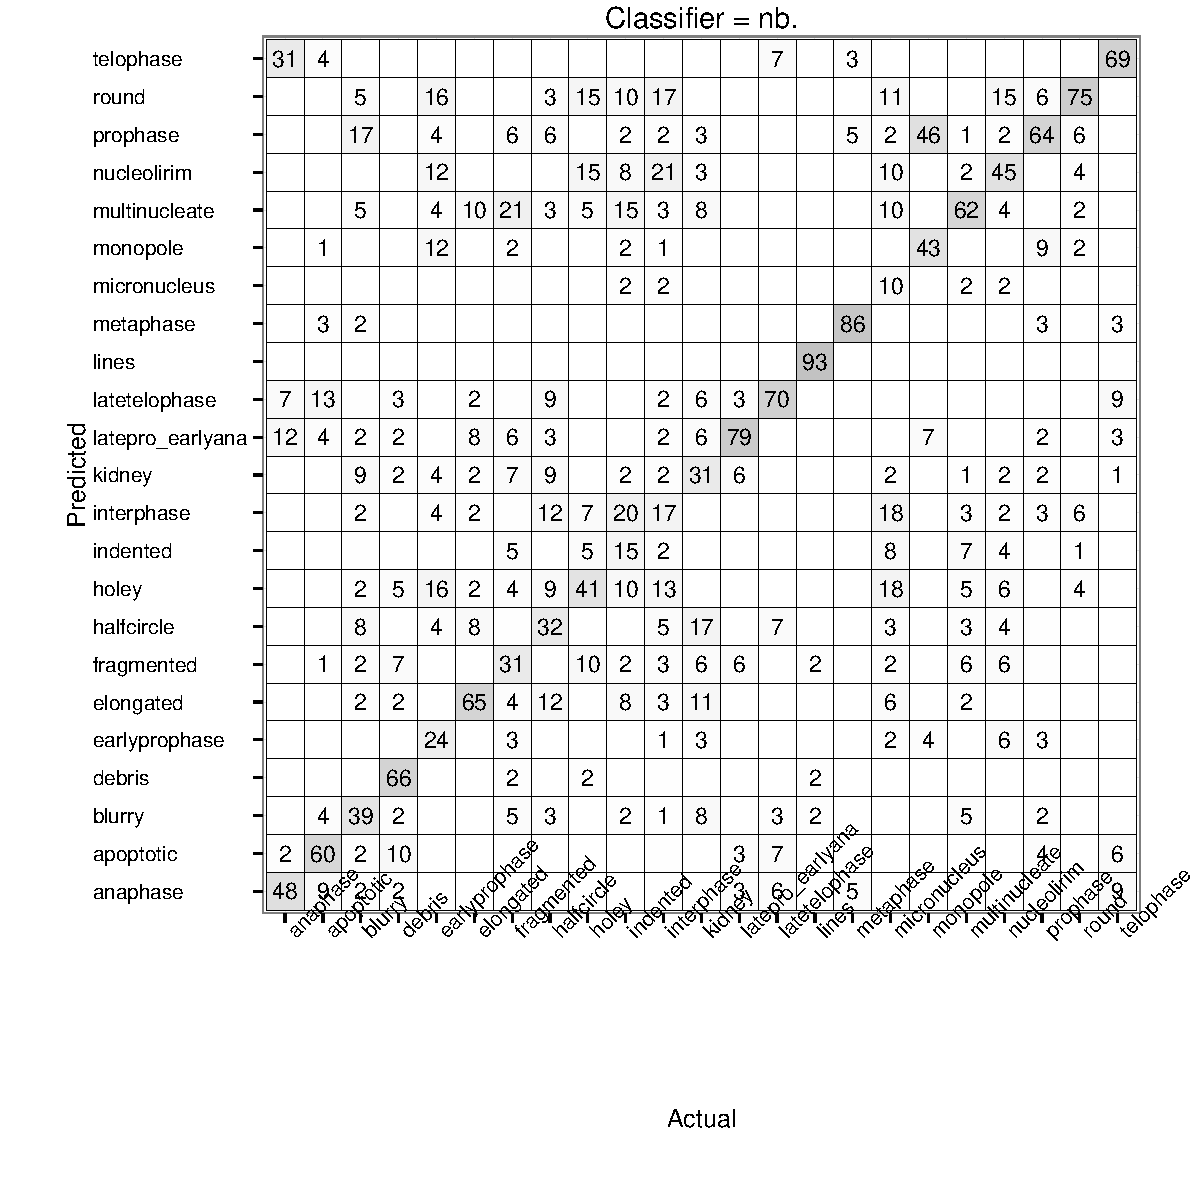
\includegraphics[width=0.8\linewidth]{confmat_loocv_nb.pdf}
\end{figure}
}
%-----------------------------
%-----------------------------
\renewcommand{\sha}{30aece85_comparison}
\graphicspath{{../results/master/\sha/}}
%-----------------------------
%-----------------------------
\frame{
\frametitle{Counts (without interphase)}
\begin{figure}
    \centering
	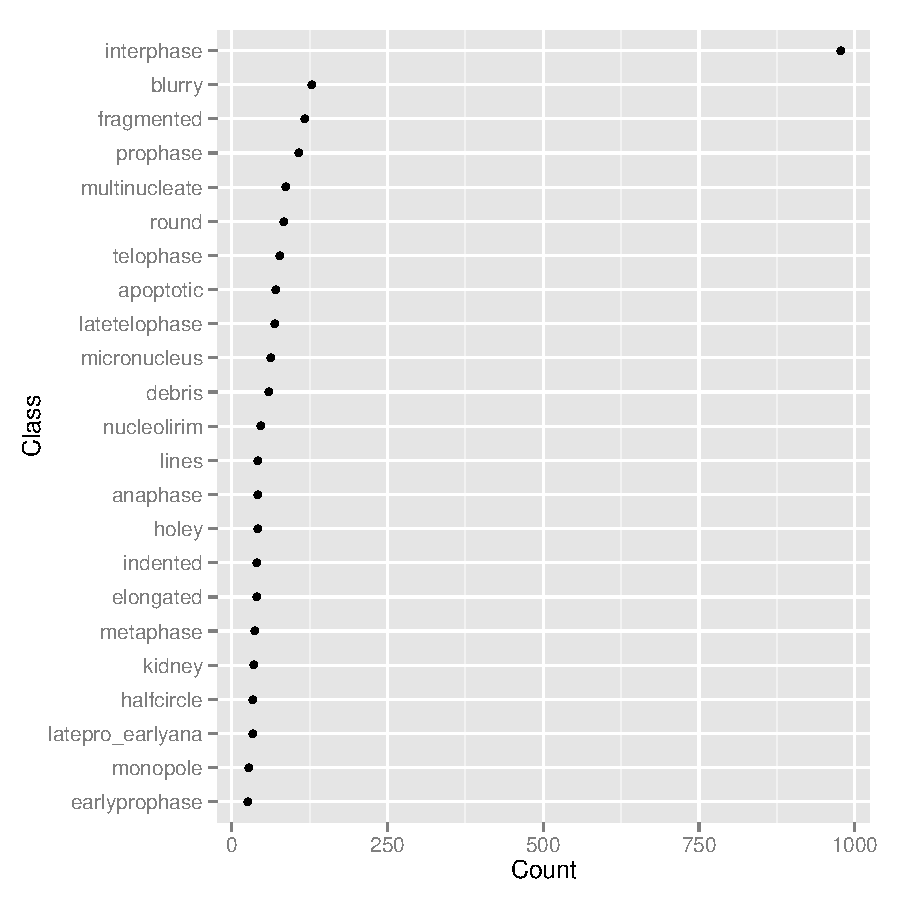
\includegraphics[width=0.8\linewidth]{counts.pdf}
\end{figure}
}
%-----------------------------
%-----------------------------
\frame{
\frametitle{\sha}
\begin{figure}
    \centering
	\includegraphics[width=0.8\linewidth]{Balanced_Accuracy_comparison.pdf}
\end{figure}
}
%-----------------------------
%-----------------------------
\frame{
\frametitle{\sha}
\begin{figure}
    \centering
	\includegraphics[width=0.8\linewidth]{Sensitivity_comparison.pdf}
\end{figure}
}
%-----------------------------


%-----------------------------
\frame{
\frametitle{Jul 17, 2013}
}
%-----------------------------

%-----------------------------
\graphicspath{{../results/master/04a4028d/}}
\renewcommand{\inputpath}[1]{../results/master/04a4028d/#1}
%-----------------------------

%-----------------------------
\frame{
\frametitle{Summary}
\begin{itemize}
\item Do leave-group-out (lgocv) and leave-one-out (loocv) analysis
\item Only Naive-Bayes (nb) for now
\item Look at confusion matirx as well as sensitivity / specificity to evaluate performance
\end{itemize}
}
%-----------------------------


\foreach \classifier in {nb}
{
\foreach \analysis in {confmat, senspec}
{


%-----------------------------
\frame{
\frametitle{\classifier : loocv }
\begin{figure}
    \centering
	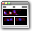
\includegraphics[width=0.8\linewidth]{\analysis_loocv_\classifier.pdf}
\end{figure}
}
%-----------------------------

%-----------------------------
\frame{
\frametitle{\classifier : lgocv }
\begin{figure}
    \centering
	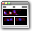
\includegraphics[width=0.8\linewidth]{\analysis_lgocv_\classifier.pdf}
\end{figure}
}
%-----------------------------


}
}




%-----------------------------
\frame{
\frametitle{Jul 15, 2013}
}
%-----------------------------

%-----------------------------
\graphicspath{{../results/master/7263fec0/}}
\renewcommand{\inputpath}[1]{../results/master/7263fec0/#1}
%-----------------------------

%-----------------------------
\frame{
\frametitle{Summary}
\begin{itemize}
\item 5-fold cross validation, 3 repetitions, across different classifiers
\end{itemize}
}
%-----------------------------

%-----------------------------
\frame{
\frametitle{Summary}
\begin{figure}
    \centering
	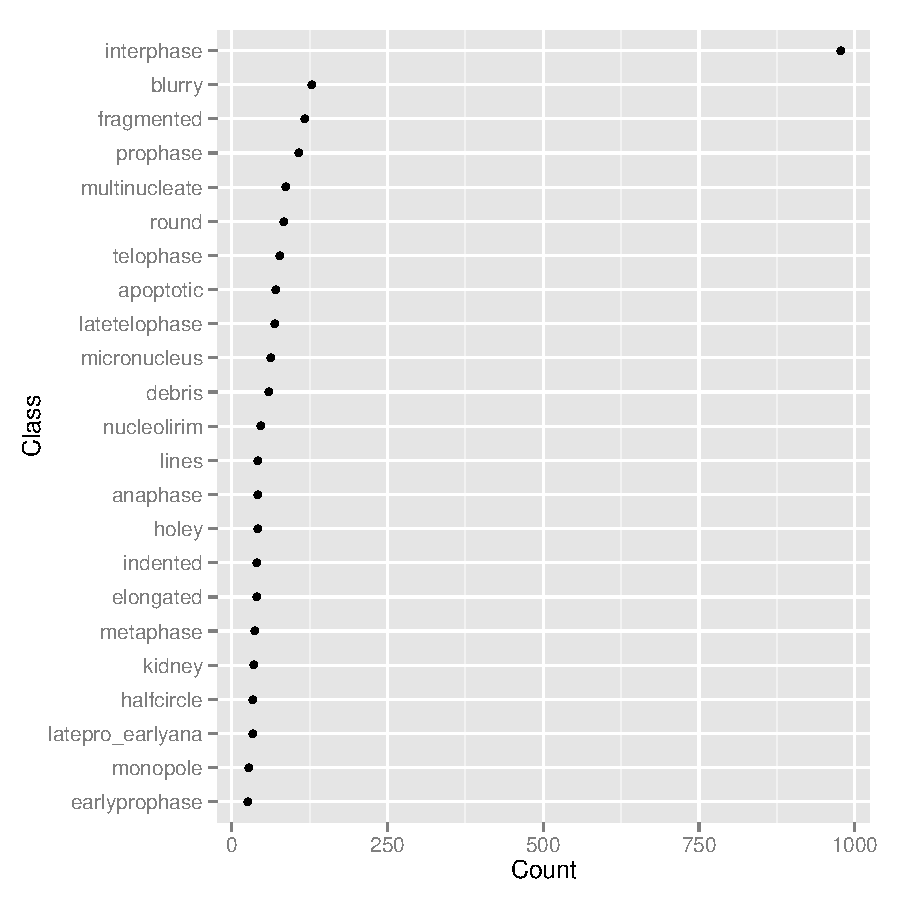
\includegraphics[width=0.8\linewidth]{counts.pdf}
\end{figure}

}
%-----------------------------

%-----------------------------
\graphicspath{{../results/master/}}
\renewcommand{\inputpath}[1]{../results/master/#1}
%-----------------------------


\foreach \classifier in {knn, lda, rf, nb}
{

%-----------------------------
\frame{
\frametitle{\classifier : confusion matrix}
\begin{figure}
    \centering
	\includegraphics[width=0.8\linewidth]{f44e1049/confmat_\classifier.pdf}
\end{figure}
}
%-----------------------------

%-----------------------------
\frame{
\frametitle{\classifier : confusion matrix (remove interphase)}
\begin{figure}
    \centering
	\includegraphics[width=0.8\linewidth]{ec662873/confmat_\classifier.pdf}
\end{figure}
}
%-----------------------------

%-----------------------------
\frame{
\frametitle{\classifier : summary}
\input{\inputpath{f44e1049/results_\classifier}}
}
%-----------------------------

%-----------------------------
\frame{
\frametitle{\classifier : summary (remove interphase) }
\input{\inputpath{ec662873/results_\classifier}}
}
%-----------------------------
}





\end{document}